\chapter{Fundamentação Teórica}
\label{cap:fundamentacao}

Este capítulo apresenta os conceitos de \english{\acrfull{csr}} e \english{\acrfull{ssr}}, abordando os princípios fundamentais do desenvolvimento web relacionados à renderização de conteúdo. Também são discutidos aspectos como \acrshort{seo}, desempenho, infraestrutura de serviços e impacto na experiência do usuário, estabelecendo a base teórica para o estudo de caso desenvolvido neste trabalho.

\section{\english{Client-Side Rendering} (\acrshort{csr})}
\label{subsec:csr}

A \textbf{\english{\acrfull{csr}}} é uma técnica em que a geração da interface e do conteúdo final ocorre diretamente no navegador do usuário, utilizando JavaScript\footnote{JavaScript é uma linguagem de programação interpretada, amplamente utilizada para adicionar interatividade e dinamismo às páginas web. Ela permite implementar funcionalidades como atualizações em tempo real, animações, mapas interativos e validações de formulários, enriquecendo a experiência do usuário. Juntamente com HTML e CSS, JavaScript compõe as três principais tecnologias da World Wide Web. Além de ser executada no navegador (\acrshort{csr}), a linguagem também pode ser utilizada no \english{\acrfull{ssr}} por meio de ambientes como Node.js(um ambiente de execução JavaScript de código aberto e multiplataforma que permite executar código JavaScript no lado do servidor, utilizando uma arquitetura orientada a eventos e não bloqueante, ideal para aplicações escaláveis e em tempo real.\cite{nodejs2025} ), possibilitando o desenvolvimento de aplicações completas com uma única linguagem.\cite{js2025}}. Nessa abordagem, o servidor envia um arquivo \english{\acrfull{html}} mínimo, contendo apenas a estrutura básica da página e referências a arquivos de estilo e scripts.{\cite{atori2024}}

Segundo \citeonline{atori2024}, o processo de renderização no cliente segue as seguintes etapas:

\begin{enumerate}
    \item O servidor envia uma página \acrshort{html} em branco contendo apenas links para os arquivos \english{\acrfull{css}} e JavaScript.
    \item O navegador interpreta o \acrshort{html} e constrói a árvore do \english{\acrfull{dom}}
    \item Os arquivos de estilo (\acrshort{css}) e script (JavaScript) são baixados pelo navegador.
    \item A aplicação é renderizada dinamicamente pelo JavaScript, incluindo elementos visuais como texto, imagens e botões.
    \item O conteúdo da página é atualizado de forma interativa conforme o usuário interage com a aplicação.
\end{enumerate}

Esse modelo é comumente utilizado em aplicações \english{\acrfull{spa}}, nas quais o carregamento inicial é seguido por atualizações dinâmicas sem recarregamento da página. Frameworks como React\footnote{React é uma biblioteca JavaScript para construção de interfaces de usuário, desenvolvida pelo Facebook. \cite{react2025} }, Vue.js\footnote{Vue.js é um framework JavaScript progressivo utilizado para a criação de interfaces web interativas, focado na camada de visualização. \cite{vue2025} }, Angular\footnote{Angular é um framework para desenvolvimento de aplicações web, mantido pelo Google, que utiliza TypeScript como linguagem principal. \cite{angular2025} } e Svelte\footnote{Svelte é um framework JavaScript que realiza a compilação de componentes no momento do build, gerando código otimizado sem a necessidade de um virtual DOM. \cite{svelte2025} } são amplamente utilizados para implementar \acrshort{csr}.

\begin{figure}[h!]
    \centering
    \caption{Etapas do método de renderização no lado do cliente}
    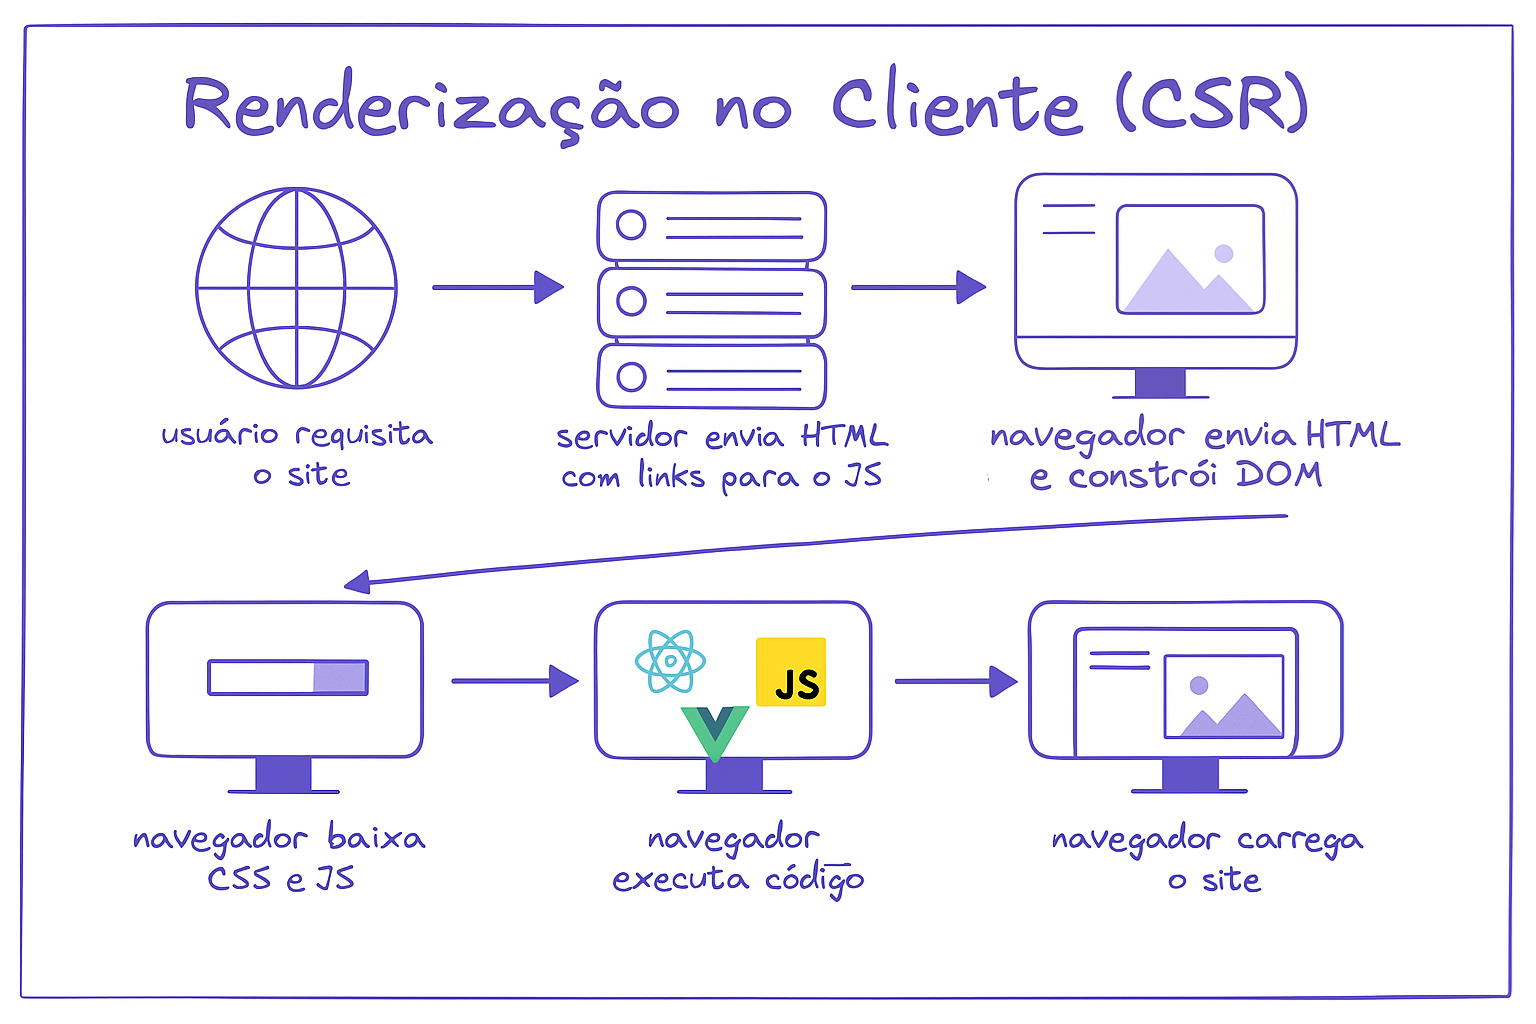
\includegraphics[width=0.9\textwidth]{media/client_side_rendering.png}
    \legend{Fonte: \cite{atori2024} (adaptado)}
    \label{fig:client_side_rendering}
\end{figure}

A \autoref{fig:client_side_rendering} ilustra visualmente o fluxo completo da renderização no lado do cliente (\acrshort{csr}). O processo é iniciado quando o usuário acessa o site em questão. Em resposta, o servidor envia o arquivo \acrshort{html} básico, contendo apenas links para os arquivos de estilo \acrshort{css} e scripts JavaScript responsáveis por carregar e renderizar o conteúdo da aplicação.

Na sequência, o navegador interpreta esse \acrshort{html} e constrói a estrutura da página por meio da árvore \acrshort{dom}. No entanto, o conteúdo principal ainda não está visível. O navegador então precisa baixar os arquivos de estilo (\acrshort{css}) e os scripts JavaScript referenciados no documento inicial.

Com os scripts carregados, o navegador executa o código JavaScript, que normalmente utiliza bibliotecas ou frameworks como React ou Vue para gerar dinamicamente o conteúdo da aplicação. Somente após essa etapa o conteúdo completo do site é finalmente exibido ao usuário, quando o navegador conclui o processo de renderização e o site é carregado completamente.

\begin{lstlisting}[language=html, capt.\ion={Exemplo de HTML mínimo em aplicação Angular com CSR}, label={lst:angular_html}]
<!DOCTYPE html>
<html lang="en">
<head>
  <meta charset="utf-8">
  <title>CryptoWebsite</title>
  <base href="/">
  <meta name="viewport" content="width=device-width, initial-scale=1">
  <link rel="icon" type="image/x-icon" href="favicon.ico">
  <style>*,*:before,*:after{margin:0;padding:0;box-sizing:border-box;
    font-family:Inter,sans-serif}html{font-size:62.5%}</style>
  <link rel="stylesheet" href="styles.9d4c7581c7242.css">
</head>
<body>
  <app-root></app-root>
  <script src="runtime.6170988ad52a05db.js" type="module"></script>
  <script src="polyfills.574970d5ec4bdb97.js" type="module"></script>
  <script src="main.202d37bb6740400e.js" type="module"></script>
</body>
</html>
\end{lstlisting}

Esse padrão é típico de aplicações \acrshort{spa}, onde todo o conteúdo é inserido dinamicamente a partir da execução dos arquivos JavaScript. O elemento \texttt{<app-root>} funciona como ponto de entrada da aplicação, sendo substituído no navegador pelos componentes definidos no framework Angular. {\cite{atori2024}}


\section{\english{Server-Side Rendering} (\acrshort{ssr})}
\label{subsec:ssr}

A \textbf{\english{\acrfull{ssr}}} é uma abordagem em que a geração do conteúdo e da interface ocorre integralmente no servidor antes de ser enviada ao navegador do cliente. Ou seja, o servidor processa a lógica da aplicação, obtém dados necessários (por exemplo, em bancos de dados ou \emph{APIs}) e retorna ao cliente um arquivo \english{\acrshort{html}} já renderizado. Dessa forma, o navegador exibe imediatamente a página completa, sem precisar executar \emph{scripts} para montar o conteúdo inicial \cite{atori2024}. 

Segundo \citeonline{atori2024}, o processo típico de renderização no lado do servidor pode ser descrito em quatro etapas principais:

\begin{enumerate}
    \item O servidor recebe uma requisição para uma página e recupera os dados necessários para compor seu conteúdo (por exemplo, produtos de uma base de dados ou artigos de um blog).
    \item O servidor insere esses dados em um \emph{template} \acrshort{html}, gerando a estrutura final da página.
    \item Em seguida, o servidor aplica estilos e finaliza a renderização, resultando em um documento \acrshort{html} completamente montado.
    \item Por fim, esse documento \acrshort{html} é enviado ao navegador do usuário, exibindo a página prontamente, sem a necessidade de executar \emph{JavaScript} durante o carregamento inicial.
\end{enumerate}

Nesse modelo, a fase de hydration\footnote{Hydration é uma etapa essencial no \acrshort{ssr}, em que o JavaScript torna interativo o conteúdo HTML previamente renderizado no servidor.} ocorre após o carregamento inicial da página. costuma ocorrer após a entrega do conteúdo estático. Significa que, assim que o arquivo \acrshort{html} é carregado e mostrado ao usuário, o \emph{JavaScript} do lado do cliente assume o controle para tratar as interações e atualizações dinâmicas subsequentes. Dessa forma, o \acrshort{ssr} beneficia tanto o primeiro acesso (tornando o conteúdo visível rapidamente) quanto o \acrshort{seo}, por exibir ao rastreador dos mecanismos de busca um código \acrshort{html} completo. \cite{atori2024}.

\begin{figure}[H]
  \centering
  \caption{Etapas do método de renderização no lado do servidor}
  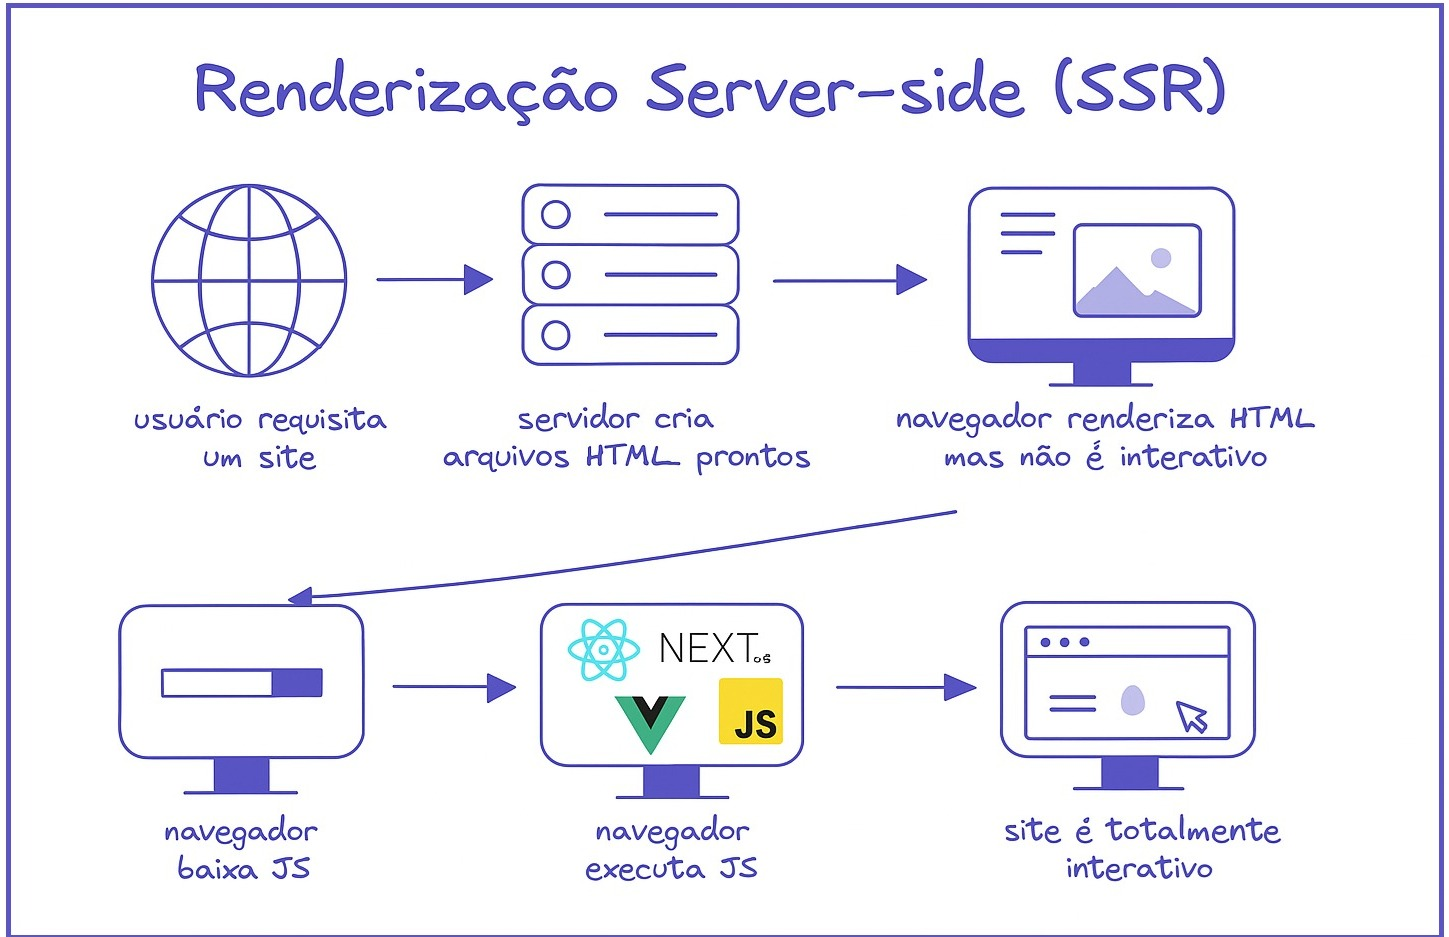
\includegraphics[width=0.8\textwidth]{media/server_side_rendering.jpeg}
  \legend{Fonte: \cite{atori2024} (adaptado)}
  \label{fig:server_side_rendering}
\end{figure}

A \autoref{fig:server_side_rendering} ilustra o fluxo de uma aplicação \acrshort{ssr}. Ao receber a requisição, o servidor gera a página completa em \acrshort{html} e a envia ao cliente. Essa estratégia costuma ser vantajosa em cenários onde o carregamento inicial rápido e a indexação por motores de busca são prioridades, como em sites de e-commerce e páginas de \emph{landing}, permitindo que o usuário visualize o conteúdo de forma imediata. 


\emph{Meta-\-frameworks}\footnote{
  Os meta-frameworks são sistemas de desenvolvimento web que operam em um nível superior a frameworks tradicionais, como React, Vue ou Svelte. Seu principal objetivo é agregar e organizar múltiplas funcionalidades comuns no desenvolvimento de aplicações, oferecendo uma estrutura mais completa e opinativa. \cite{benHolmes}
} como \emph{Next.js}\footnote{Next.js é um framework de código aberto para React que facilita a criação de aplicações web com renderização no lado do servidor (\acrshort{ssr}) e geração de sites estáticos. Fornece recursos como roteamento baseado em arquivos, pré-renderização e suporte a APIs. \cite{nextjs2024}} , \emph{Nuxt.js}\footnote{Nuxt.js é um framework baseado em Vue.js que simplifica a criação de aplicações universais, oferecendo renderização no lado do servidor, geração de sites estáticos e uma arquitetura modular que facilita a escalabilidade. \cite{nuxtjs2024}} , \emph{SvelteKit}\footnote{SvelteKit é um framework para Svelte que oferece uma experiência de desenvolvimento simplificada, permitindo a criação de aplicações com renderização no lado do servidor e no cliente, além de otimizações de desempenho. \cite{sveltekit2024}} , \emph{Angular Universal}\footnote{Angular Universal é a solução oficial de renderização no lado do servidor para aplicações Angular, permitindo a renderização de páginas no servidor para melhorar o desempenho e a indexação por mecanismos de busca. \cite{angularuniversal2024}} , \emph{Remix}\footnote{Remix é um framework full-stack para React que foca na experiência do desenvolvedor e no desempenho, oferecendo renderização no lado do servidor e um modelo de dados baseado em carregadores e ações. \cite{remix2024}} , \emph{Astro}\footnote{Astro é um framework moderno que permite a construção de sites rápidos, carregando apenas o JavaScript necessário e permitindo o uso de componentes de diferentes frameworks como React, Svelte e Vue. \cite{astro2024}} e \emph{Qwik}\footnote{Qwik é um framework JavaScript que introduz o conceito de aplicações web "resumíveis", visando tempos de carregamento instantâneos e desempenho aprimorado, utilizando renderização no lado do servidor e aprimoramentos progressivos. \cite{qwik2024}} são amplamente utilizados para construir aplicações com suporte a \acrshort{ssr}, simplificando a configuração e fornecendo recursos prontos para lidar com roteamento, recuperação de dados e \english{hidration}.

No \autoref{lst:nextjs_html}, pode-se observar que o arquivo \acrshort{html} já contém todo o \emph{markup} necessário para exibir o conteúdo da página. Assim que o navegador recebe esse arquivo, o usuário já visualiza o cabeçalho, o texto e o layout definidos. Posteriormente, o \emph{JavaScript} baixado (por exemplo, \texttt{main.js}) pode entrar em ação para lidar com eventos, rotas adicionais e atualizações dinâmicas, caso o desenvolvedor deseje funcionalidades mais interativas.

Por fim, aplicações \acrshort{ssr} tendem a apresentar melhor performance em termos de \emph{time-to-first-byte}\footnote{O \emph{time-to-first-byte} (TTFB) é uma métrica que mede o tempo decorrido entre o envio de uma solicitação HTTP pelo cliente e o recebimento do primeiro byte da resposta do servidor. Um TTFB menor indica maior rapidez na resposta do servidor, impactando diretamente na velocidade de carregamento da página e na experiência do usuário. \cite{ttfb-craig}} e de \emph{indexabilidade}\footnote{A \emph{indexabilidade} refere-se à capacidade dos motores de busca de rastrear e indexar o conteúdo de uma página web. Aplicações SSR, ao fornecerem conteúdo totalmente renderizado no servidor, facilitam a indexação eficiente pelos motores de busca, melhorando a visibilidade nos resultados de pesquisa. \cite{ttfb-oskay}} por motores de busca, ao mesmo tempo em que podem demandar maior carga de processamento no servidor. A escolha por \acrshort{ssr} ou não, portanto, depende do perfil da aplicação e das prioridades do projeto, considerando fatores como volume de tráfego, necessidade de interatividade e requisitos de otimização de conteúdo.

\begin{lstlisting}[language=html, caption={Exemplo de HTML mínimo em aplicação Next.js com SSR}, label={lst:nextjs_html}]
<!DOCTYPE html>
<html lang="en">
<head>
  <meta charset="utf-8">
  <title>My SSR App</title>
  <meta name="viewport" content="width=device-width, initial-scale=1">
  <style>
    /* Exemplo simples de estilo inline */
    body {
      margin: 0;
      font-family: Arial, sans-serif;
      background: #f6f6f6;
    }
    h1 { color: #333; }
  </style>
</head>
<body>
  <!-- Conteúdo já processado e inserido no servidor -->
  <div id="__next">
    <header>
      <h1>Olá, mundo!</h1>
    </header>
    <main>
      <p>Este conteúdo foi renderizado no servidor usando Next.js.</p>
    </main>
  </div>
  <!-- Scripts do Next.js para interação no cliente -->
  <script src="/_next/static/chunks/main.js" defer></script>
</body>
</html>
\end{lstlisting}



\section{Fundamentos de Desenvolvimento Web}
\label{sec:fundamentos-devweb}
Para entender como as abordagens \acrshort{ssr} e \acrshort{csr} se inserem no cenário de desenvolvimento web, é fundamental revisar protocolos, modelos de arquitetura e ferramentas.

\subsection{Protocolo HTTP}
\label{subsec:http}
O \textbf{Protocolo de Transferência de Hipertexto} (\acrshort{http}) define como clientes (navegadores) e servidores comunicam-se na web. Na \acrshort{ssr}, cada solicitação aciona a geração dinâmica da página no servidor.JavaScript é uma linguagem de programação interpretada utilizada para criar conteúdo dinâmico em Já na \acrshort{csr}, o cliente requisita recursos (HTML mínimo, JavaScript, CSS) e efetua chamadas subsequentes ao servidor para buscar dados adicionais via \textit{APIs}, geralmente no formato \textit{JSON}.

Evoluções como HTTP/2 e HTTP/3 trouxeram melhorias de desempenho (multiplexação de requisições, compressão de cabeçalhos, etc.), impactando positivamente o tempo de carregamento tanto em \acrshort{ssr} quanto em \acrshort{csr}.

\subsection{Modelos de Arquitetura Web}
\label{subsec:modelos-arq-web}
Os modelos arquiteturais variam conforme os requisitos de escalabilidade, manutenção e desempenho:

\begin{itemize}
    \item \textbf{Arquitetura Monolítica}: Um único projeto concentra \textit{frontend} e \textit{backend}, frequentemente usando \acrshort{ssr}. Possui inicialização simples, mas pode tornar-se complexo de manter e escalar.
    \item \textbf{Microserviços}: Divide a aplicação em múltiplos serviços independentes. Cada serviço pode escolher a melhor abordagem de renderização (SSR ou CSR), facilitando a escalabilidade seletiva.
    \item \textbf{Serverless}: As funções são executadas sob demanda em plataformas de nuvem, onde a renderização pode ocorrer tanto no servidor (funções que retornam HTML) quanto no cliente (ao entregar apenas APIs).
\end{itemize}

\subsection{Ferramentas e \textit{Frameworks}}
\label{subsec:ferramentas-frameworks}
O ecossistema de desenvolvimento web oferece diversas ferramentas que simplificam \acrshort{ssr} e \acrshort{csr}:

\begin{itemize}
    \item \textbf{\acrshort{ssr}}: \textit{Next.js} (React), \textit{Nuxt.js} (Vue), \textit{SvelteKit} (Svelte), entre outros.
    \item \textbf{\acrshort{csr}}: React, Vue.js, Angular e muitas bibliotecas voltadas para \textit{Single Page Applications} (SPA).
\end{itemize}


\section{Infraestrutura de Serviço Web}
\label{sec:infraestrutura-web}

A decisão por \acrshort{ssr} ou \acrshort{csr} influencia diretamente a infraestrutura necessária:

\begin{itemize}
    \item \textbf{Servidores e Processamento}: Em \acrshort{ssr}, o servidor gera páginas dinamicamente, aumentando a carga de CPU. Já em \acrshort{csr}, o servidor atua mais como um provedor de arquivos estáticos e APIs.
    \item \textbf{\english{Content Delivery Networks} (CDNs)}: Tanto para SSR quanto para CSR, uma CDN pode melhorar a distribuição de arquivos estáticos (HTML, CSS, JavaScript, imagens) e reduzir a latência.
    \item \textbf{Escalabilidade}: Aplicações com alto número de requisições precisam de estratégias adequadas para lidar com picos de acesso. Em \acrshort{ssr}, muitas requisições simultâneas podem sobrecarregar o servidor; em \acrshort{csr}, o foco está em serviços de dados e na entrega eficiente de arquivos iniciais.
\end{itemize}

\textbf{Segurança} também se faz presente em ambas as abordagens. Boas práticas incluem:
\begin{itemize}
    \item Uso de \textbf{HTTPS} para proteger a comunicação.
    \item Implementação de \textbf{CORS} (Cross-Origin Resource Sharing) quando necessário.
    \item Tratamento de \textbf{tokens de sessão/autenticação} com cuidado para evitar vazamento de dados.
\end{itemize}

---

\section{Experiência do Usuário (\english{User Experience} – UX)}
\label{sec:ux}
Um dos objetivos principais ao optar por \acrshort{ssr} ou \acrshort{csr} é oferecer uma experiência de usuário satisfatória. Alguns aspectos relevantes incluem:

\begin{itemize}
    \item \textbf{Tempo de Carregamento Inicial}: Em \acrshort{ssr}, o conteúdo aparece mais rápido para o usuário no primeiro acesso. Em \acrshort{csr}, embora o primeiro carregamento possa ser mais lento (devido ao download e execução de scripts), a navegação interna torna-se mais rápida após a aplicação já estar carregada no navegador.
    \item \textbf{Interatividade e Navegação}: \acrshort{csr} geralmente proporciona transições fluidas entre páginas e atualizações em tempo real sem recarregamento completo. \acrshort{ssr}, porém, pode recorrer a estratégias de atualização parcial, como AJAX, para melhorar a interatividade.
    \item \textbf{Acessibilidade}: Independentemente da abordagem, a aplicação deve atender a boas práticas de acessibilidade, garantindo que leitores de tela e outras tecnologias assistivas consigam interpretar adequadamente o conteúdo.
    \item \textbf{Consistência de Interface}: A aplicação deve manter uma experiência coesa, independentemente de páginas estarem sendo renderizadas no servidor ou no cliente.
\end{itemize}

\subsection{\english{Search Engine Optimization} (SEO)}
\label{sec:seo}
O \textbf{\acrshort{seo}} é o conjunto de técnicas para melhorar o ranqueamento de um site nos resultados dos mecanismos de busca. No contexto de \acrshort{csr} e \acrshort{ssr}, o \acrshort{seo} é especialmente importante por afetar:

\begin{itemize}
    \item \textbf{Indexação de Conteúdo}: No \acrshort{ssr}, o HTML completo chega aos robôs de busca, facilitando a indexação imediata. Já em \acrshort{csr}, se o robô não executar JavaScript, pode ocorrer indexação incompleta ou ausente.
    \item \textbf{Metadados Dinâmicos}: O uso de títulos, descrições e tags \textit{Open Graph} deve ser planejado para gerar conteúdo correto em cada rota, principalmente em aplicações SPA.
    \item \textbf{Velocidade de Carregamento}: O tempo de carregamento é um fator relevante no ranqueamento, exigindo otimizações como \textit{caching}, minificação de scripts, compressão de imagens e \textit{lazy loading}.
\end{itemize}

Alguns mecanismos de busca modernos suportam \textit{renderização dinâmica} (executando JavaScript para rastrear páginas em CSR), mas configurações incorretas podem prejudicar a visibilidade do site nos resultados de pesquisa.

---

---

\noindent
Conclui-se, portanto, que \acrshort{ssr} e \acrshort{csr} oferecem caminhos distintos para a criação de aplicações web, cada qual com implicações em termos de desempenho, \acrshort{seo}, infraestrutura e experiência do usuário. Nas próximas seções deste trabalho, será apresentado um estudo de caso prático que visa comparar e avaliar as duas abordagens em diferentes cenários de uso.

\label{s2}


